\documentclass[tikz, crop]{standalone}

\usepackage{amsmath}

\usetikzlibrary{arrows.meta, shapes.geometric, positioning}
\tikzset{%
  >={Latex[width=2mm,length=2mm]},
  % Specifications for style of nodes:
        base/.style = {rectangle, rounded corners, draw=black,
                           minimum width=4cm, minimum height=1cm,
                           text centered, font=\sffamily},
       if/.style = {diamond, draw=black,
                           fill=blue!20},
        term/.style = {ellipse, draw=blue!50!black,
                           fill=blue!40},
        process/.style = {base, minimum width=2.5cm, fill=blue!5,
                           font=\ttfamily},
        line/.style = {draw},
        point/.style={circle}
}

\newcommand{\init}{
    \begin{tabular}{l}
        $s=0$\\
        $\delta=k$\\
        $\mathbf{X}=\mathrm{LSQ}(\tau', A)$\\
        $\chi^2=\mathrm{chisq}(\tau', \mathbf{X})$\\
        $\chi^2_o=\chi^2$\\
    \end{tabular}
}
\newcommand{\iterate}{
    \begin{tabular}{l}
        $s_o=s$\\
        $n = n+1$\\
        $s_+=s+\delta$\\
        $s_-=s-\delta$\\
        $\tau_+ = \mathrm{shift}(\tau', s_+)$\\
        $\tau_- = \mathrm{shift}(\tau', s_-)$\\
        $\mathbf{X_+}=\mathrm{LSQ}(\tau'_+, A)$\\
        $\mathbf{X_-}=\mathrm{LSQ}(\tau'_-, A)$\\
        $\chi^2_+=\mathrm{chisq}(\tau'_+, \mathbf{X}_+)$\\
        $\chi^2_-=\mathrm{chisq}(\tau'_-, \mathbf{X}_-)$\\
        $\chi^2=\min(\chi^2_+, \chi^2_-)$\\
    \end{tabular}
}

\newcommand{\criteria}{
    \begin{tabular}{l}
        $n < n_{lim}$\\
        \textbf{\&\&}\\
        $\chi^2 > \chi^2_{min}$\\
    \end{tabular}
}

\newcommand{\chisq}{
    \begin{tabular}{l}
        $\chi^2 < \chi^2_o$
    \end{tabular}
}

\newcommand{\newshift}{
    \begin{tabular}{l}
       $s=s_o$\\
       $\delta = 0.1 \cdot \delta$\\
    \end{tabular}
}

\begin{document}
% Drawing part, node distance is 1.5 cm and every node
% is prefilled with white background
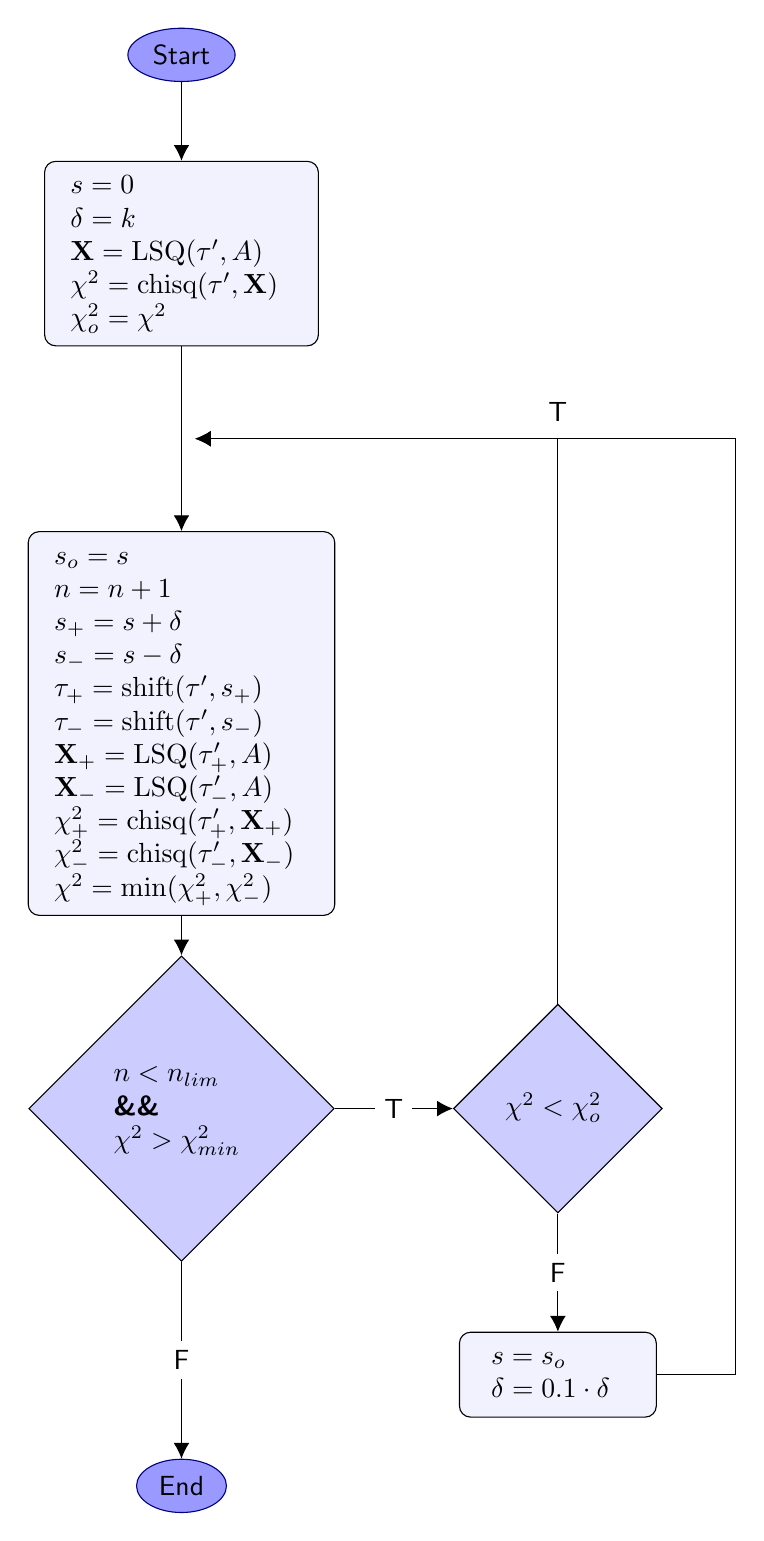
\begin{tikzpicture}[node distance=1.5cm,
    every node/.style={fill=white, font=\sffamily}, align=center]
  % Specification of nodes (position, etc.)
    \node (start)              [term]{Start};
    \node (init)         [process, below=10mm of start] {\init};
    \node (point)       [point, below=10mm of init]{};
    \node (iterate)         [process, below=10mm of point] {\iterate};
    \node(criteria)     [if, below=5mm of iterate] {\criteria};
    \node(chisq)     [if, right=1.5cm of criteria] {\chisq};
    \node(newShift) [process, below=1.5cm of chisq]{\newshift};
    \node (end)         [term, below=2.5cm of criteria]{End};

  % Specification of lines between nodes specified above
  % with aditional nodes for description 
  \draw[->]             (start) -- (init);
  \draw[->]     (init) -- (iterate);
  \draw[->]     (iterate) -- (criteria);
  \draw[->]      (criteria) -- node{F}(end);
  \draw[->]      (criteria) -- node{T}(chisq);
  \draw[->]      (chisq) -- node{F}(newShift);
  \draw[->]      (chisq) |-node[above=.1cm of chisq]{T} (point);
  \draw[->]      (newShift.east) --++(1cm, 0)|- (point.east);
  % \draw[->]     (onResumeBlock) -- (activityRuns);
  % \draw[->]      (activityRuns) -- node[text width=4cm]
  %                                  {Another activity comes in
  %                                   front of the activity} (onPauseBlock);
  % \draw[->]      (onPauseBlock) -- node {The activity is no longer visible}
  %                                  (onStopBlock);
  % \draw[->]       (onStopBlock) -- node {The activity is shut down by
  %                                  user or system} (onDestroyBlock);
  % \draw[->]    (onRestartBlock) -- (onStartBlock);
  % \draw[->]       (onStopBlock) -| node[yshift=1.25cm, text width=3cm]
  %                                  {The activity comes to the foreground}
  %                                  (onRestartBlock);
  % \draw[->]    (onDestroyBlock) -- (ActivityDestroyed);
  % \draw[->]      (onPauseBlock) -| node(priorityXMemory)
  %                                  {higher priority $\rightarrow$ more memory}
  %                                  (ActivityEnds);
  % \draw           (onStopBlock) -| (priorityXMemory);
  % \draw[->]     (ActivityEnds)  |- node [yshift=-2cm, text width=3.1cm]
  %                                   {User navigates back to the activity}
  %                                   (onCreateBlock);
  % \draw[->] (onPauseBlock.east) -- ++(2.6,0) -- ++(0,2) -- ++(0,2) --                
  %    node[xshift=1.2cm,yshift=-1.5cm, text width=2.5cm]
  %    {The activity comes to the foreground}(onResumeBlock.east);
  \end{tikzpicture}
\end{document}
